\chapter{ច្បាប់ទី១ទែម៉ូឌីណាមិច}
\section{ប្រព័ន្ធទែម៉ូឌីណាមិចៈ}
\begin{definition}
	\begin{enumerate}[m]
		\item \emph{ប្រព័ន្ធៈ} គឺជាវត្ថុ ឬសំណុំវត្ថុដែលយើងលើកមកសិក្សា ដោយធៀបទៅនឹងវត្ថុដ៏ទៃផ្សេងទៀត។\\(វត្ថុដ៏ទៃផ្សេងទៀតនោះ យើងហៅថាៈ មជ្ឈដ្ឋានក្រៅ)។
		\item \emph{ភាពនៃប្រព័ន្ធៈ} គឺជាសំណុំលេខដែលវាស់ទំហំរូបវិទ្យា ដើម្បីសម្គាល់ប្រព័ន្ធនៅខណៈណាមួយ មានមាឌ សម្ពាធ និងសីតុណ្ហភាពជាអថេរសម្គាល់ភាពនៃប្រព័ន្ធ ។
		\item \emph{បម្លែងទែម៉ូឌីណាមិចៈ} ប្រព័ន្ធមួយទទួលបម្លែងទែម៉ូឌីណាមិច កាលណាវាផ្លាស់ប្តូរភាព ដោយប្តូរតែ កម្មន្ត និងកម្តៅ ជាមួយមជ្ឈដ្ឋានក្រៅប៉ុណ្ណោះ។ គេចែកបម្លែងទែម៉ូឌីណាមិចជាពីរគឺ បម្លែងចំហ និងបម្លែងបិទ។
		\begin{itemize}
			\item [$\ast$] បម្លែងចំហ-បម្លែងបិទៈ ពេលប្រព័ន្ធមួយទទួលបម្លែងទែម៉ូឌីណាមិចៈ
			\begin{itemize}
				\item បើភាពដើម និងភាពស្រេចនៃប្រព័ន្ធមួយ ខុសគ្នា នោះគេថាប្រព័ន្ធទទួលរងនូវបម្លែចំហ។
				\item បើភាពដើម និងភាពស្រេចនៃប្រព័ន្ធមួយ ដូចគ្នា នោះគេថាប្រព័ន្ធទទួលរងនូវបម្លែងបិទ។
			\end{itemize}
		\end{itemize}
	\item \emph{ប្រព័ន្ធទែម៉ូឌីណាមិចៈ} គឺជាប្រព័ន្ធដែលទទួល បម្លែងទែម៉ូឌីណាមិចដោយមានការផ្លាស់ប្តូរភាពដើម និងភាពស្រេចតាមដំណើរប្រព្រឹត្តទៅខុសៗគ្នា។
	\begin{itemize}
		\item សមីការប្រែប្រួលភាពនៃឧស្ម័នបរិសុទ្ធៈ $\frac{P_1V_1}{T_1}=\frac{P_2V_2}{T_2}=nR=$ ថេរ\\
		ដែលភាពដើម $P_1,V_1$ សម្ពាធ និងមាឌឧស្ម័ននៅសីតុណ្ហភាព $T_1$ និង ភាពស្រេច $P_2,V_2$ សម្ពាធ និងមាឌឧស្ម័ននៅសីតុណ្ហភាព $T_2$ មាឌគិតជា $m^{3}$ សីតុណ្ហភាពគិតជា $K$ និងសម្ពាធគិតជា $Pa$\\($V_1, V_2$ អាចគិតជា $L$ ក៏បាន)។
	\end{itemize}
	\end{enumerate}
\end{definition}
\section{កម្មន្តបំពេញក្នុងពេលបម្រែបម្រួលមាឌៈ}
\subsection{ករណីសម្ពាធថេរ(លំនាំអុីសូបារ):}
ឧបមាថាឧស្ម័នមានមាឌដើម $V_{i}$ ស្ថិតក្នុងសុីឡាំងដែលមានមុខកាត់ $A$ បិទជិតដោយពីស្តុងមួយ។\\ ពេលឧស្ម័នរុញពីស្តុងពីទីតាំង $x_{i}$ ទៅទីតាំង $x_{f}$ ដែល $V_{i}=Ax_{i}$ និង $V_{f}=Ax_{f}$ ក្រោមសម្ពាធថេរ $P_{o}:$
\begin{figure}[H]
	\caption{លំនាំអុីសូបារ}
		\begin{subfigure}[t]{.5\textwidth}
			\centering
			\begin{tikzpicture}[yscale=.85]
			\node [draw, cylinder, cylinder uses custom fill, cylinder body fill=gray!20, 
			cylinder end fill=gray!70, shape aspect=4, rotate=0, minimum width=3cm] (c1) at 
			(1.3,0){};
			\node [draw, cylinder, cylinder uses custom fill, cylinder body fill=gray!20, 
			cylinder end fill=gray!70, shape aspect=4, rotate=0, minimum width=3cm] (c2) at 
			(-1,0){};
			
			\node [draw, cylinder, cylinder body fill=gray!50, 
			cylinder end fill=gray!50, shape aspect=4, rotate=0, minimum height=6.7cm, minimum 
			width=3cm] (c) {};
			
			\draw[<->] (-3,2.8)--(1.3,2.8);
			\draw[|-] (-3,-2)--(5,-2);
			\draw[dashed] (-3,2.8) -- (-3,0);
			\draw[dashed] (1.3,2.8) -- (1.3,1.5);
			\draw[<->] (-3,2)--(-1,2);
			\draw[dashed] (-1,2) -- (-1,1.5);
			\draw[-] (4.5,0) node { \color{blue}\text{ពីស្តុង} } (4,0)--(2,0);
			\draw (4.9,-2.3) node {$x$};
			\draw (1.3,-2.3) node {$x_{f}$};
			\draw[dashed] (1.3,-2) -- (1.3,-1.5);
			\draw (1.3,-2) node {$\bullet$};
			\draw (-1,-2.3) node {$x_{i}$};
			\draw[dashed] (-1,-2) -- (-1,-1.5);
			\draw (-1,-2) node {$\bullet$};
			
			\draw [line width=3pt, arrows = {-Latex[width=10pt,length=10pt]}] (-.5, 0) -- (.5, 0);
			
			\coordinate [label=$P_{0}$] ($P_{0}$) at (-2,-.3);
			\coordinate [label=$V_{i}$] ($V_{i}$) at (-2,2);
			\coordinate [label=$V_{f}$] ($V_{f}$) at (-.5,2);
		\end{tikzpicture}
		\subcaption{\koc កម្មន្តបំពេញដោយឧស្ម័ន}
	\end{subfigure}
	%
	\begin{subfigure}[t]{.5\textwidth}
		\centering
		\begin{tikzpicture}[scale=1.35]
		\begin{scope}
		\fill [orange!60!white] (1,0) -- (1,2) -- (3,2) -- (3,0) -- cycle;
		\pattern[pattern color=white,pattern=bricks] (1,0) -- (1,2) -- (3,2) -- (3,0) -- cycle;
		\coordinate (O) at (0, 0);
		\coordinate (P) at (0, 2.7);
		\draw (0,0)-- (4,0);
		\draw [dashed] (0,2)-- (2,2);
		\draw [thick] (1,2)-- (3,2);
		\draw [dashed] (1,2)-- (1,0);
		\draw [dashed] (3,2)-- (3,0);
		\draw (0,0)-- (0,3);
		\draw (2,1) node {\kml \color{magenta}ក្រឡាផ្ទៃ};
		\draw [->, >=Latex] (2,2) -- (2.1,2);
		\draw (1,2) node {$\bullet$};
		\draw (1,2) node [color=blue, above]{$A$};
		\draw (3,2) node [color=blue, above]{$B$};
		\draw (3,2) node {$\bullet$};
		\draw(0,2.9) node [color=blue, left=.1cm]{$P$};
		\draw(0,2) node [color=blue, left=.1cm]{$P_{o}$};
		\draw(4,0) node [color=blue, right=.1cm]{$V$};
		\draw(1,-0.2) node [color=blue]{$V_{i}$};
		\draw(3,-0.2) node [color=blue]{$V_{f}$};
		\draw(4,0) node [color=blue, right=.1cm]{$V$};
		\end{scope}
		\end{tikzpicture}
		\subcaption{\koc ដ្យាក្រាម $\left(P-V\right)$}
	\end{subfigure}
\end{figure}
\begin{definition}
	\emph{លំនាំអុីសូបារ {\en(Isobaric Process)}} គឺជាលំនាំមួយដែលសម្ពាធនៃប្រព័ន្ធក្នុងបម្លែងទែម៉ូឌីណាមិចមានតម្លៃថេរ។
\end{definition}
\begin{enumerate}[m]
	\item \emph{\kml កម្មន្តបំពេញដោយឧស្ម័ន:}
		\begin{align*}
		\text{កម្មន្តបំពេញដោយឧស្ម័ន}\quad :&\quad  W=F\times\Delta x=F\left(x_{f}-x_{i}\right)\\
		\text{ដែល}\quad :&\quad P_{o}=\frac{F}{A}\quad \text{នោះ}\quad F=P_{o}A\\
		\text{យើងបាន}\quad :&\quad W=P_{o}A\left(x_{f}-x_{i}\right)=P_{o}\left(Ax_{f}-Ax_{i}\right)\\
		\text{នាំឲ្យ}\quad :&\quad W=P_{o}\left(V_{f}-V_{i}\right)=P_{o}\Delta V\\
		\text{ដូចនេះ}\quad :&\quad W=P_{o}\Delta V
		\end{align*}
	\item \emph{\kml សមីការប្រែប្រួលភាពៈ} $\frac{P_{1}V_{1}}{T_{1}}=\frac{P_{2}V_{2}}{T_{2}}$
	\begin{itemize}
		\item \emph{ករណីសម្ពាធថេរៈ} $P_{1}=P_{2}=P_{o}=$ ថេរ
		\begin{align*}
			\text{យើងបាន}\quad :&\quad \frac{V_{1}}{T_{1}}=\frac{V_{2}}{T_{2}}=ឮ\text{ថេរ}\\
			\text{នាំឲ្យ}\quad :&\quad V_{2}=\left(\frac{V_{1}}{T_{1}}\right)T_{2}\quad \text{មានរាង}\quad y=ax\quad \text{ជាបន្ទាត់}
		\end{align*}
		\item \emph{កម្មន្តក្នុងលំនាំអុីសូបារៈ} តាមដ្យាក្រាម $\left(P-V\right)$ ក្នុងរូបបង្ហាញពីសម្ពាធថេរ និងកំណើនមាឌនៃឧស្ម័នៈ\\ $W=P\Delta V=P\left(V_{f}-V_{i}\right)=A$\\
		ដូចនេះក្នុងដ្យាក្រាម $\left(P-V\right)$ កម្មន្តដែលបំពេញ ដោយឧស្ម័នគឺជាក្រឡាផ្ទៃចតុកោណកែងដែលមានវិមាត្រជា\\ $P$ និង $\Delta V$។
	\end{itemize}
	\item \emph{\kml ដ្យាក្រាម $\left(P-V\right),~\left(P-T\right)$ និង $\left(V-T\right)$}
	\begin{figure}[H]
		\caption{ដ្យាក្រាម}
		\begin{subfigure}[t]{.3\textwidth}
			\centering
			\begin{tikzpicture}[scale=1]
			\begin{scope}
				\fill [orange!60!white] (1,0) -- (1,2) -- (3,2) -- (3,0) -- cycle;
				\pattern[pattern color=white,pattern=bricks] (1,0) -- (1,2) -- (3,2) -- (3,0) -- cycle;
				\coordinate (O) at (0, 0);
				\coordinate (P) at (0, 2.7);
				\draw (0,0)-- (4,0);
				\draw [dashed] (0,2)-- (2,2);
				\draw [thick] (1,2)-- (3,2);
				\draw [dashed] (1,2)-- (1,0);
				\draw [dashed] (3,2)-- (3,0);
				\draw (0,0)-- (0,3);
				\draw(0,2.9) node [color=blue, left=.1cm]{$P$};
				\draw [->,>=Latex] (2,2) -- (2.1,2);
				\draw(0,2) node [color=blue, left=.1cm]{$P_{o}$};
				\draw(4,0) node [color=blue, right=.1cm]{$V$};
				\draw(1,-.3) node [color=blue]{$V_{i}$};
				\draw(3,-.3) node [color=blue]{$V_{f}$};
				\draw(4,0) node [color=blue, right=.1cm]{$V$};
				\draw (1,2) node {$\bullet$};
				\draw (1,2) node [color=blue, above]{$A$};
				\draw (3,2) node [color=blue, above]{$B$};
				\draw (3,2) node {$\bullet$};
				\node[right,text=blue](I) at (0,3){$ \displaystyle W=P\left(V_{f}-V_{i}\right)$};
				\draw[->](2,.5) to[out=0,in=0] (I);
			\end{scope}
			\end{tikzpicture}
			\subcaption{\koc ដ្យាក្រាម $\left(P-V\right)$}
		\end{subfigure}
		%
		\begin{subfigure}[t]{.3\textwidth}
			\centering
			\begin{tikzpicture}[scale=1]
			\begin{scope}
			\draw [->,>=Latex] (2,2) -- (2.1,2);
			\draw (0,0)-- (4,0);
			\draw [dashed] (0,2)-- (2,2);
			\draw (1,2)-- (3,2);
			\draw [dashed] (1,2)-- (1,0);
			\draw [dashed] (3,2)-- (3,0);
			\draw (0,0)-- (0,3);
			\draw(0,2.9) node [color=blue, left=.1cm]{$P$};
			\draw(0,2) node [color=blue, left=.1cm]{$P_{o}$};
			\draw(4,0) node [color=blue, right=.1cm]{$T$};
			\draw(1,-.3) node [color=blue]{$T_{i}$};
			\draw(3,-.3) node [color=blue]{$T_{f}$};
			\draw (1,2) node {$\bullet$};
			\draw (1,2) node [color=blue, above]{$A$};
			\draw (3,2) node [color=blue, above]{$B$};
			\draw (3,2) node {$\bullet$};
			\end{scope}
			\end{tikzpicture}
			\subcaption{\koc ដ្យាក្រាម $\left(P-T\right)$}
		\end{subfigure}
		\begin{subfigure}[t]{.3\textwidth}
		\centering
		\begin{tikzpicture}[scale=1]
		\begin{scope}
			\draw (0,0)-- (4,0);
			\draw [dashed] (0,0.5)-- (1,0.5);
			\draw [dashed] (0,2)-- (3,2);
			\draw (1,0.5)-- (3,2);
			\draw [dashed] (1,0.5)-- (1,0);
			\draw [dashed] (3,2)-- (3,0);
			\draw (0,0)-- (0,3);
			\draw(0,2.9) node [color=blue, left=.1cm]{$V$};
			\draw(0,0.5) node [color=blue, left=.1cm]{$V_{i}$};
			\draw(0,2) node [color=blue, left=.1cm]{$V_{f}$};
			\draw(4,0) node [color=blue, right=.1cm]{$T$};
			\draw(1,-.3) node [color=blue]{$T_{i}$};
			\draw(3,-.3) node [color=blue]{$T_{f}$};
			\draw (1,0.5) node {$\bullet$};
			\draw (1,0.5) node [color=blue, above]{$A$};
			\draw (3,2) node [color=blue, above]{$B$};
			\draw (3,2) node {$\bullet$};
		\end{scope}
		\end{tikzpicture}
		\subcaption{\koc ដ្យាក្រាម $\left(V-T\right)$}
		\end{subfigure}
	\end{figure}
\end{enumerate}
\subsection{ករណីសម្ពាធប្រែប្រួលស្មើ}
\quad បើប្រព័ន្ធប្រែប្រួលសម្ពាធពី $P_{1}$ ទៅ $P_{2}$ យើងបានសម្ពាធមធ្យមកំណត់ដោយៈ $P_{av}=\frac{P_{1}+P_{2}}{2}$
	\begin{enumerate}[m]
		\item \emph{\kml កម្មន្តបំពេញដោយឧស្ម័ន}
		\begin{align*}
		\text{យើងបាន}\quad :&\quad W=P_{av}\Delta V=\frac{P_1+P_2}{2}\Delta V\\
		\text{ម្យ៉ាងទៀត}\quad :&\quad W=\frac{2P_1-P1+P2}{2}\Delta V
		\end{align*}
		\begin{align*}
		\text{នោះ}\quad :&\quad W=P_{1}\Delta V+\frac{P_{2}-P_{1}}{2}\Delta V\\
		\text{ដូចនេះ}\quad :&\quad W=P_{1}\Delta V+\frac{1}{2}\left(P_{2}-P_{1}\right)\Delta V
		\end{align*}
		\item \emph{\kml ដ្យាក្រាម $\left(P-V\right)$ ករណីសម្ពាធប្រែប្រួលស្មើ}
		\begin{figure}[H]
			\centering
			\begin{tikzpicture}[scale=1.5]
				\begin{scope}
				\fill [orange!60!white] (1,0) -- (1,2) -- (3,2) -- (3,0) -- cycle;
				\pattern[pattern color=white,pattern=bricks] (1,0) -- (1,2) -- (3,2) -- (3,0) -- cycle;
				\fill [red!80!orange] (1,2) -- (3,3) -- (3,2) -- cycle;
				\pattern[pattern color=white,pattern=bricks] (1,2) -- (3,3) -- (3,2) -- cycle;
				\draw (0,0)-- (4,0);
				\draw [dashed] (0,2)-- (2,2);
				\draw [dashed] (0,3)-- (3,3);
				\draw [dashed] (1,2)-- (3,2);
				\draw [thick] (1,2)-- (3,3);
				\draw [dashed] (3,2)-- (3,3);
				\draw [dashed] (1,2)-- (1,0);
				\draw [dashed] (3,2)-- (3,0);
				\draw (0,0)-- (0,4);
				\draw(0,3.9) node [color=blue, left=.1cm]{$P$};
				\draw(0,2) node [color=blue, left=.1cm]{$P_{1}$};
				\draw(0,3) node [color=blue, left=.1cm]{$P_{2}$};
				\draw(4,0) node [color=blue, right=.1cm]{$V$};
				\draw(1,-.3) node [color=blue]{$V_{1}$};
				\draw(3,-.3) node [color=blue]{$V_{2}$};
				\draw(4,0) node [color=blue, right=.1cm]{$V$};
				\draw (1,2) node {$\bullet$};
				\draw (1,2) node [color=blue, above]{$A$};
				\draw (3,3) node [color=blue, above]{$B$};
				\draw (3,2) node [color=blue, right]{$C$};
				%\draw (3,2) node {$\bullet$};
				\draw (3,3) node {$\bullet$};
				\node[right,text=blue](I) at (3,2.8){$ \displaystyle W_{1}=A_{ABC}$};
				\draw[->](2,2.3) to[out=0,in=0] (I);
				\node[right,text=blue](II) at (3,1){$ \displaystyle W_{2}=A_{BCV_{2}V_{1}}$};
				\draw[->](2,.5) to[out=0,in=0] (II);
				\end{scope}
			\end{tikzpicture}
			\caption{ដ្យាក្រាម $\left(P-V\right)$ ករណីសម្ពាធប្រែប្រួលស្មើ}
		\end{figure}
	\item \emph{\kml កម្មន្តក្នុងករណីសម្ពាធ​សមាមាត្រនឹងមាឌ}\\
	\quad តាមដ្យាក្រាម $\left(P-V\right)$ ខាងលើ យើបានក្រឡាផ្ទៃឆូតនៃ $\left(P-V\right)$ គឺ $A=A_{ABC}+A_{BCV_{2}V_{1}}$\\
	\begin{align*}
		\text{ដែល}\quad :&\quad A_{ABC}=\frac{1}{2}\left(P_2-P_1\right)\left(V_2-V_1\right)\quad \text{និង}\quad A_{BCV_2V_1}=P_1\Delta V\\
		\text{សមមូល}\quad :&\quad A=P_1\Delta V +\frac{1}{2}\left(P_2-P_1\right)\left(V_2-V_1\right)\\
		\text{ដូចនេះ}\quad :&\quad A=W=P_1\Delta V +\frac{1}{2}\left(P_2-P_1\right)\Delta V
	\end{align*}
	ដូចនេះកម្មន្តដែលបំពេញដោយឧស្ម័ន គឺជាក្រឡាផ្ទៃផ្នែកឆូតដែលបានខ័ណ្ឌដោយខ្សែកោង $\left(P-V\right)$។
	\end{enumerate}
	\subsection{ករណីសីតុណ្ហភាពថេរ(លំនាំអុីសូទែម):}

	\quad ក្នុងករណីប្រព័ន្ធដំណើរការដោយរក្សាសីតុណ្ហភាពថេរ តាមពិសោធន៍គេបានដ្យាក្រាម $\left(P-V\right)$ ដូចរូបៈ
		\begin{figure}[H]
			\caption{លំនាំអុីសូទែម}
			\begin{subfigure}[t]{.5\textwidth}
				\centering
				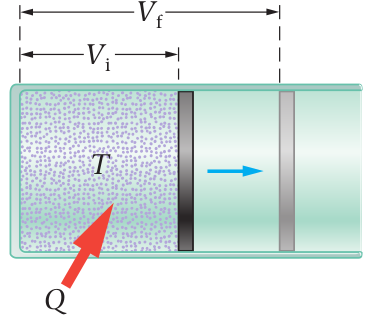
\includegraphics[scale=0.40]{07}
				\subcaption{\koc សុីឡាំងដែលមានសីតុណ្ហភាពថេរ}
			\end{subfigure}
		\begin{subfigure}[t]{.5\textwidth}
			\centering
			\begin{tikzpicture}[scale=1.3]
			\begin{scope}
			\coordinate [label=left:$O$] (O) at (0,0);
			\draw [blue] (O);
			\draw (0.8,2.5) .. controls (1.5,1) .. (3.5,0.5);
			%\fill [red!80!orange]
			(1,2) .. controls (1,1.5) .. (3,0);
			%\pattern[pattern color=white,pattern=bricks]
			(1,2) .. controls (1,1.5) .. (3,0);
			\draw (0,0)-- (4,0);
			\draw [dashed] (0,2)-- (1,2);
			\draw [dashed] (0,.6)-- (3,.6);
			\draw [dashed] (1,2)-- (1,0);
			\draw [dashed] (3,0.6)-- (3,0);
			\draw (0,0)-- (0,3);
			\draw(0,2.9) node [color=blue, left=.1cm]{$P$};
			\draw(0,2) node [color=blue, left=.1cm]{$P_{f}$};
			\draw(0,0.6) node [color=blue, left=.1cm]{$P_{i}$};
			\draw(4,0) node [color=blue, right=.1cm]{$V$};
			\draw(1,-.3) node [color=blue]{$V_{i}$};
			\draw(3,-.3) node [color=blue]{$V_{f}$};
			\draw (1,2) node {$\bullet$};
			\draw (1,2) node [color=blue, right=.2cm]{$A$};
			\draw (3,.5) node [color=blue, above=0.2cm]{$B$};
			\draw (3,.6) node {$\bullet$};
			\end{scope}
			\end{tikzpicture}
			\subcaption{\koc ដ្យាក្រាម $\left(P-V\right)$ ករណីសីតុណ្ហភាពថេរ}
		\end{subfigure}
		\end{figure}
	\begin{definition}
		\emph{លំនាំអុីសូទែម{\en (Isothermal Process):}} គឺជាលំនាំមួយដែលសីតុណ្ហភាពនៃប្រព័ន្ធក្នុងបម្លែងទែម៉ូឌីណាមិចមានតម្លៃថេរ។
	\end{definition}
	\begin{enumerate}[m]
		\item \emph{\kml កម្មន្តបំពេញដោយឧស្ម៏នៈ}
		\begin{align*}
		\text{តាមសម្រាយបញ្ជាក់ខាងលើៈ}\quad :&\quad W=A\quad \text{ដែល}\quad W=A=\int_{V_{i}}^{V_{f}}pdV=Nk_{B}T\int_{V_{i}}^{V_{f}}\frac{dV}{V}\\
		\text{នោះ}\quad :&\quad W=Nk_{B}T\ln\left[V\right]^{V_{f}}_{V_{i}}\\
		\text{នាំឲ្យៈ}\quad :& \quad W=Nk_{B}T\ln\left(\frac{V_f}{V_{i}}\right)=nRT\left(\frac{V_{f}}{V_{i}}\right)\\
		\text{ដូចនេះ}\quad :&\quad W=nRT\left(\frac{V_{f}}{V_{i}}\right)
		\end{align*}
		\item \emph{\kml សមីការប្រែប្រួលភាពៈ} $\frac{P_{1}V_{1}}{T_{1}}=\frac{P_{2}V_{2}}{T_{2}}$
		\begin{itemize}
			\item \emph{ករណីសីតុណ្ហភាពថេរៈ} $T_{1}=T_{2}=$ ថេរ 
			\begin{align*}
				\text{យើងបាន}\quad :&\quad P_{1}V_{1}=P_{2}T_{2}=\text{ថេរ}\\
				\text{នាំឲ្យ}\quad :&\quad P_{2}=\frac{P_1V_{1}}{V_2}\quad \text{មានរាង}\quad y=\frac{a}{x}\quad \text{ជាអុីពែបូល}
			\end{align*}
			\item \emph{កម្មន្តក្នុងករណីសីតុណ្ហភាពថេរៈ} 
			\begin{align*}
					\text{យើងមាន}\quad :&\quad W=nRT\ln\left(\frac{V_{f}}{V_{i}}\right)\quad \text{ឬ}\quad W=Nk_{B}T\ln\left(\frac{V_{f}}{V_{i}}\right)\\
					\text{ដែល}\quad:&\quad \frac{V_{f}}{V_{i}}=\frac{P_{i}}{P_{f}}\\
					\text{នោះ}\quad :&\quad W=nRT\ln\left(\frac{P_{i}}{P_{f}}\right)\quad\text{ឬ}\quad W=P_{i}V_{i}\ln\left(\frac{P_{i}}{P_{f}}\right)
			\end{align*}
		\end{itemize}
		\item \emph{\kml ដ្យាក្រាម $\left(P-V\right),~\left(T-V\right)$ និង $\left(P-T\right)$}
		\begin{figure}[H]
			\caption{ដ្យាក្រាម}
			\begin{subfigure}[t]{.3\textwidth}
				\centering
				\begin{tikzpicture}[scale=1]
					\begin{scope}
						\draw (0.8,2.5) .. controls (1.5,1) .. (3.5,0.5);
						%\fill [red!80!orange]
						(1,2) .. controls (1,1.5) .. (3,0);
						%\pattern[pattern color=white,pattern=bricks]
						(1,2) .. controls (1,1.5) .. (3,0);
						\draw (0,0)-- (4,0);
						\draw [dashed] (0,2)-- (1,2);
						\draw [dashed] (0,.6)-- (3,.6);
						\draw [dashed] (1,2)-- (1,0);
						\draw [dashed] (3,0.6)-- (3,0);
						\draw (0,0)-- (0,3);
						\draw(0,2.9) node [color=blue, left=.1cm]{$P$};
						\draw(0,2) node [color=blue, left=.1cm]{$P_{f}$};
						\draw(0,0.6) node [color=blue, left=.1cm]{$P_{i}$};
						\draw(4,0) node [color=blue, right=.1cm]{$V$};
						\draw(1,-.3) node [color=blue]{$V_{i}$};
						\draw(3,-.3) node [color=blue]{$V_{f}$};
						\draw (1,2) node {$\bullet$};
						\draw (1,2) node [color=blue, right=.2cm]{$A$};
						\draw (3,.5) node [color=blue, above=0.2cm]{$B$};
						\draw (3,.6) node {$\bullet$};
					\end{scope}
				\end{tikzpicture}
				\subcaption{\koc ដ្យាក្រាម $\left(P-V\right)$}
			\end{subfigure}
			\begin{subfigure}[t]{.3\textwidth}
				\centering
				\begin{tikzpicture}[scale=1]
				\begin{scope}
				\draw [->] (2,2) -- (2.1,2);
				\draw (0,0)-- (4,0);
				\draw [dashed] (0,2)-- (2,2);
				\draw (1,2)-- (3,2);
				\draw [dashed] (1,2)-- (1,0);
				\draw [dashed] (3,2)-- (3,0);
				\draw (0,0)-- (0,3);
				\draw(0,2.9) node [color=blue, left=.1cm]{$T$};
				\draw(0,2) node [color=blue, left=.1cm]{$T_{o}$};
				\draw(4,0) node [color=blue, right=.1cm]{$V$};
				\draw(1,-.3) node [color=blue]{$V_{i}$};
				\draw(3,-.3) node [color=blue]{$V_{f}$};
				\draw (1,2) node {$\bullet$};
				\draw (1,2) node [color=blue, above]{$A$};
				\draw (3,2) node [color=blue, above]{$B$};
				\draw (3,2) node {$\bullet$};
				\end{scope}
				\end{tikzpicture}
				\subcaption{\koc ដ្យាក្រាម $\left(T-V\right)$}
			\end{subfigure}
			\begin{subfigure}[t]{.3\textwidth}
				\centering
				\begin{tikzpicture}[scale=1]
				\begin{scope}
				\draw (0,0)-- (4,0);
				\draw [dashed] (0,2)-- (2,2);
				\draw [thick] (2,0.5)-- (2,2);
				\draw [dashed] (0,0.5)-- (2,0.5);
				\draw [dashed] (2,0)-- (2,0.5);
				\draw (0,0)-- (0,3);
				\draw(0,2.9) node [color=blue, left=.1cm]{$P$};
				\draw [->] (2,1) -- (2,1.5);
				\draw(0,2) node [color=blue, left=.1cm]{$P_{f}$};
				\draw(0,0.5) node [color=blue, left=.1cm]{$P_{i}$};
				\draw(4,0) node [color=blue, right=.1cm]{$T$};
				\draw(2,-.3) node [color=blue]{$T_{i}=T_{f}$};
				\draw(4,0) node [color=blue, right=.1cm]{$T$};
				\draw (2,0.5) node {$\bullet$};
				\draw (2,0.5) node [color=blue, right]{$A$};
				\draw (2,2) node [color=blue, above]{$B$};
				\draw (2,2) node {$\bullet$};
				\end{scope}
				\end{tikzpicture}
				\subcaption{\koc ដ្យាក្រាម $\left(P-T\right)$}
			\end{subfigure}
		\end{figure}
	\end{enumerate}\newpage
	\subsection{ករណីមាឌថេរ(លំនាំអុីសូករ)}
	\begin{figure}[H]
		\caption{លំនាំអុីសូករ}
		\begin{subfigure}[t]{.5\textwidth}
			\centering
			\begin{tikzpicture}[>=stealth, shape aspect=.5]
			\node [cylinder,cylinder uses custom fill, cylinder end fill=yellow!20,
			cylinder body fill=cyan!15!white, shape border rotate=90, minimum width=2cm, minimum
			height=2.8cm, aspect=2.5, overlay, draw] {};
			\draw[opacity=0.25] (-1,-.8) arc (180:0:1cm and 0.5cm);
			\fill[gray] (0,-.72) circle [x radius=.9cm, y radius=0.35cm];
			\draw (0,0) node {$P_{i}$};
			%
			\draw (3,0) node [cylinder,cylinder uses custom fill, cylinder end fill=yellow!20,
			cylinder body fill=cyan!15!white, shape border rotate=90, minimum width=2cm, minimum
			height=2.8cm, aspect=2.5, overlay, draw] {};
			\draw[opacity=0.25] (2,-.8) arc (180:0:1cm and 0.5cm);
			\fill[gray] (3,-.72) circle [x radius=.9cm, y radius=0.35cm];
			\draw (2.5,.7) node {$Q$};
			\draw [red!75,  line width=1cm/4, ->] (1.5,-.5) -- (2.5,.5);
			%
			\draw (6,0) node [cylinder,cylinder uses custom fill, cylinder end fill=yellow!20,
			cylinder body fill=cyan!15!white, shape border rotate=90, minimum width=2cm, minimum
			height=2.8cm, aspect=2.5, overlay, draw] {};
			\draw[opacity=0.25] (5,-.8) arc (180:0:1cm and 0.5cm);
			\fill[gray] (6,-.72) circle [x radius=.9cm, y radius=0.35cm];
			\draw (6,0) node {$P_{f}$};
			\end{tikzpicture}
			\subcaption{\koc សុីឡាំងមានមាឌថេរ}
		\end{subfigure}
		\begin{subfigure}[t]{.5\textwidth}
			\centering
			\begin{tikzpicture}[scale=1]
			\begin{scope}
			\draw (0,0)-- (4,0);
			\draw [dashed] (0,2)-- (2,2);
			\draw [thick] (2,0.5)-- (2,2);
			\draw [dashed] (0,0.5)-- (2,0.5);
			\draw [dashed] (2,0)-- (2,0.5);
			\draw (0,0)-- (0,3);
			\draw(0,2.9) node [color=blue, left=.1cm]{$P$};
			\draw [->] (2,1) -- (2,1.5);
			\draw(0,2) node [color=blue, left=.1cm]{$P_{f}$};
			\draw(0,0.5) node [color=blue, left=.1cm]{$P_{i}$};
			\draw(4,0) node [color=blue, right=.1cm]{$V$};
			\draw(2,-.3) node [color=blue]{$V_{i}=V_{f}$};
			\draw(4,0) node [color=blue, right=.1cm]{$V$};
			\draw (2,0.5) node {$\bullet$};
			\draw (2,0.5) node [color=blue, right]{$A$};
			\draw (2,2) node [color=blue, above]{$B$};
			\draw (2,2) node {$\bullet$};
			\end{scope}
			\end{tikzpicture}
			\subcaption{\koc ដ្យាក្រាម $\left(P-V\right)$}
		\end{subfigure}
	\end{figure}
	\begin{definition}
		\emph{លំនាំអុីសូករ {\en (Isochoric Process):}} គឺជាលំនាំមួយដែលមាឌនៃប្រព័ន្ធក្នុងបម្លែងទែម៉ូឌីណាមិចមានតម្លៃថេរ។
	\end{definition}
	\begin{enumerate}[m]
		\item \emph{\kml កម្មន្តបំពេញដោយឧស្ម័នៈ}
		\begin{align*}
			\text{ដោយ}\quad :&\quad V_{i}=V_{f}=\text{ថេរ}\\
			\text{ដូចនេះ}\quad :&\quad W=0
		\end{align*}
		\item \emph{\kml សមីការប្រែប្រួលភាព} $\frac{P_{1}V_{_1}}{T_{1}}=\frac{P_2V_2}{T_2}$
		\begin{itemize}
			\item \emph{ករណីមាឌថេរៈ} $V_{1}=V_{2}=$ ថេរ 
			\begin{align*}
			\text{យើងបាន}\quad :&\quad \frac{P_{1}}{T_{1}}=\frac{P_{2}}{T_{2}}=\text{ថេរ}\\
			\text{នាំឲ្យ}\quad :&\quad P_{2}=\frac{P_1}{T_1}T_{2}\quad \text{មានរាង}\quad y=ax\quad \text{ជាបន្ទាត់}
			\end{align*}
		\end{itemize}
		\item \emph{\kml ដ្យាក្រាម $\left(P-V\right),~\left(T-V\right)$ និង $\left(P-T\right)$}
	\begin{figure}[H]
		\caption{ដ្យាក្រាម}
		\begin{subfigure}[t]{.3\textwidth}
			\centering
			\begin{tikzpicture}[scale=1]
			\begin{scope}
			\draw (0,0)-- (4,0);
			\draw [dashed] (0,2)-- (2,2);
			\draw [thick] (2,0.5)-- (2,2);
			\draw [dashed] (0,0.5)-- (2,0.5);
			\draw [dashed] (2,0)-- (2,0.5);
			\draw (0,0)-- (0,3);
			\draw(0,2.9) node [color=blue, left=.1cm]{$P$};
			\draw [->] (2,1) -- (2,1.5);
			\draw(0,2) node [color=blue, left=.1cm]{$P_{f}$};
			\draw(0,0.5) node [color=blue, left=.1cm]{$P_{i}$};
			\draw(4,0) node [color=blue, right=.1cm]{$V$};
			\draw(2,-.3) node [color=blue]{$V_{i}=V_{f}$};
			\draw(4,0) node [color=blue, right=.1cm]{$V$};
			\draw (2,0.5) node {$\bullet$};
			\draw (2,0.5) node [color=blue, right]{$A$};
			\draw (2,2) node [color=blue, above]{$B$};
			\draw (2,2) node {$\bullet$};
			\end{scope}
			\end{tikzpicture}
			\subcaption{\koc ដ្យាក្រាម $\left(P-V\right)$}
		\end{subfigure}
		%
		\begin{subfigure}[t]{.3\textwidth}
			\centering
			\begin{tikzpicture}[scale=1]
			\begin{scope}
			\draw (0,0)-- (4,0);
			\draw [dashed] (0,2)-- (2,2);
			\draw [thick] (2,0.5)-- (2,2);
			\draw [dashed] (0,0.5)-- (2,0.5);
			\draw [dashed] (2,0)-- (2,0.5);
			\draw (0,0)-- (0,3);
			\draw(0,2.9) node [color=blue, left=.1cm]{$T$};
			\draw [->] (2,1) -- (2,1.5);
			\draw(0,2) node [color=blue, left=.1cm]{$T_{f}$};
			\draw(0,0.5) node [color=blue, left=.1cm]{$T_{i}$};
			\draw(4,0) node [color=blue, right=.1cm]{$V$};
			\draw(2,-.3) node [color=blue]{$V_{i}=V_{f}$};
			\draw(4,0) node [color=blue, right=.1cm]{$V$};
			\draw (2,0.5) node {$\bullet$};
			\draw (2,0.5) node [color=blue, right]{$A$};
			\draw (2,2) node [color=blue, above]{$B$};
			\draw (2,2) node {$\bullet$};
			\end{scope}
			\end{tikzpicture}
			\subcaption{\koc ដ្យាក្រាម $\left(T-V\right)$}
		\end{subfigure}
		\begin{subfigure}[t]{.3\textwidth}
			\centering
			\begin{tikzpicture}[scale=1]
			\begin{scope}
			\draw (0,0)-- (4,0);
			\draw [dashed] (0,0.5)-- (1,0.5);
			\draw [dashed] (0,2)-- (3,2);
			\draw (1,0.5)-- (3,2);
			\draw [dashed] (1,0.5)-- (1,0);
			\draw [dashed] (3,2)-- (3,0);
			\draw (0,0)-- (0,3);
			\draw(0,2.9) node [color=blue, left=.1cm]{$P$};
			\draw(0,0.5) node [color=blue, left=.1cm]{$P_{i}$};
			\draw(0,2) node [color=blue, left=.1cm]{$P_{f}$};
			\draw(4,0) node [color=blue, right=.1cm]{$T$};
			\draw(1,-.3) node [color=blue]{$T_{i}$};
			\draw(3,-.3) node [color=blue]{$T_{f}$};
			\draw (1,0.5) node {$\bullet$};
			\draw (1,0.5) node [color=blue, above]{$A$};
			\draw (3,2) node [color=blue, above]{$B$};
			\draw (3,2) node {$\bullet$};
			\end{scope}
			\end{tikzpicture}
			\subcaption{\koc ដ្យាក្រាម $\left(P-T\right)$}
		\end{subfigure}
	\end{figure}
	\end{enumerate}
	\newpage
\section{ថាមពលក្នុងនៃច្បាប់ទី១ ទែម៉ូឌីណាមិច}
\subsection{កម្តៅ និងកម្មន្តៈ} \quad កម្តៅមានទំនាក់ទំនងជាមួយសីតុណ្ហភាព។ ថាមពលកម្តៅអាចផ្ទេរពីអង្គធាតុមួយទៅអង្គធាតុមួយទៀតកាលណាវាមានសីតុណ្ហភាពខុសគ្នា។ ដូចនេះសីតុណ្ហភាពខុសគ្នាជាលក្ខណៈចាំបាច់សម្រាប់ផ្ទេរកម្តៅ។\\
\subsection{ថាមពលក្នុងនៃឧស្ម័ន}
\begin{enumerate}[k]
	\item \emph{\kml ថាមពលក្នុងនៃឧស្ម័នៈ}
	\begin{definition}
		\emph{ថាមពលក្នុងនៃឧស្ម័នៈ} គឺជាថាមពលសុីនេទិចសរុបនៃម៉ូលេគុលឧស្ម័ន។
		\begin{align*}
			\text{គេកំណត់សរសេរដោយៈ}\quad :&\quad U=\frac{3}{2}Nk_{B}T=\frac{3}{2}nRT=\frac{3}{2}PV
		\end{align*}
	\end{definition}
	\item \emph{\kml បម្រែបម្រួលថាមពលក្នុងនៃឧស្ម័នៈ} បើពេលមានបម្រែបម្រួលសីតុណ្ហភាព នោះឧស្ម័នមានបម្រែបម្រួលថាមពលក្នុងៈ 
	\begin{align*}
		\text{យើងបាន}\quad :&\quad \Delta U= U_{2}-U_1\\
		\text{ដែល}\quad :&\quad U_1=\frac{3}{2}Nk_{B}T_{1}=\frac{3}{2}nRT_{1}\quad \text{និង}\quad U_{2}=\frac{3}{2}Nk_{B}T_{2}=\frac{3}{2}nRT_{2}\\
		\text{សមមូល}\quad :&\quad \Delta U=\frac{3}{2}Nk_{B}T_{2}-\frac{3}{2}Nk_{B}T_{1}\quad\text{ឬ}\quad \Delta U=\frac{3}{2}nRT_{2}-\frac{3}{2}nRT_{1}\\
		\text{ដូចនេះ}\quad :&\quad \Delta U=\frac{3}{2}Nk_{B}\Delta T=\frac{3}{2}nR\Delta T\quad \text{ឬ}\quad \Delta U=\frac{3}{2}\left(P_{2}V_{2}-P_{1}V_{1}\right)
	\end{align*}
	\begin{remark}
		បើឧស្ម័នមានសីតុណ្ហភាពថេរ នោះមិនមានបម្រែបម្រួលថាមពលក្នុងទេ ព្រោះថាមពលក្នុងអាស្រ័យនឹងសីតុណ្ហភាព។
		\begin{align*}
			\text{យើងបាន}\quad :&\quad \Delta T=T_2-T_1=0\\
			\text{ដូចនេះ}\quad :&\quad \Delta U=0
		\end{align*}
	\end{remark}
\end{enumerate}
\subsection{ច្បាប់ទី១​ទែម៉ូឌីណាមិចៈ}
\begin{definition}
	\emph{ច្បាប់ទីមួយទែម៉ូឌីណាមិចៈ} ក្នុងបម្លែងទែម៉ូឌីណាមិចកម្តៅស្រូបដោយប្រព័ន្ធស្មើនឹងផលបូកកម្មន្តបង្កើតឡើងដោយប្រព័ន្ធ និងបម្រែបម្រួលថាមពលក្នុងនៃប្រព័ន្ធ។
	\begin{align*}
		\text{គេសរសេរ}\quad :&\quad Q= W+ \Delta U
	\end{align*}
\end{definition}
\begin{remark}
	\begin{itemize}
		\item [$\ast$] {\emph{\kml សិក្សាសញ្ញាៈ}}
		\begin{enumerate}[m]
			\item បើប្រព័ន្ធបញ្ចេញកម្មន្ត(បំពេញកម្មន្ត) ឬ ធ្វើកម្មន្ត នោះ $W>0$ តែបើប្រព័ន្ធរងកម្មន្ត ឬទទួលកម្មន្ត នោះ $W<0$
			\item បើប្រព័ន្ធស្រួបកម្តៅ នោះ $Q>0$ តែបើប្រព័ន្ធបញ្ចេញកម្តៅ នោះ $Q<0$
			\item បើថាមពលក្នុងនៃប្រព័ន្ធកើន $\Delta U>0$ តែបើថាមពលក្នុងនៃប្រព័ន្ធថយចុះ នោះ $\Delta U<0$
		\end{enumerate}
	\end{itemize}
\end{remark}
\subsection{បម្លែងបិទ$\sim$គោលការណ៍សមមូលៈ}
\begin{enumerate}[m]
	\item {\emph{\kml បម្លែងបិទៈ​}} បើប្រព័ន្ធមួយប្រែប្រួលពីភាព $1$ ទៅភាព $2$ រួចត្រឡប់ពីភាព $2$ ទៅភាព $1$ វិញនោះយើងបានៈ
	\begin{itemize}
		\item ក្នុងលំនាំនៃភាព $1$ ទៅភាព $2$\quad $Q_{1}=W_{1}+\Delta U_{1}$ ឬ $Q_{1}=W_{1}+ U_{2}-U_{1}$
		\item ក្នុងលំនាំនៃភាព $2$ ទៅភាព $1$\quad $Q_{2}=W_{2}+\Delta U_{2}$ ឬ $Q_{2}=W_{2}+ U_{1}-U_{2}$
	\end{itemize}
	\begin{align*}
	\text{យើងបានបម្លែងសរុបគឺៈ}\quad :&\quad Q_{1}+Q_{2}=W_{1}+U_{2}-U_{1}+W_{2}+U_{1}-U_{2}\\
	\text{តាង}\quad :&\quad W=W_{1}+W_{2}\quad \text{នឹង}\quad Q=Q_{1}+Q_2\\
	\text{សមមូល}\quad :&\quad Q=W+0\left(\Delta U=0\right)\\
	\text{ដូចនេះ}\quad :&\quad \Delta U=Q-W=0
	\end{align*}
	\item \emph{\kml គោលការណ៍សមមូលៈ} កាលណាប្រព័ន្ធធ្វើបម្លែងបិទ ក្នុងមួយសិុច(វដ្ត) ដោយប្រព័ន្ធប្តូរតែកម្មន្ត \\និងកម្តៅជាមួយមជ្ឍដ្ឋានក្រៅ មានន័យថាៈ
	\begin{itemize}
		\item បើប្រព័ន្ធបំពេញកម្មន្ត ឬធ្វើកម្មន្ត $\left(W>0\right)$ នោះវាបញ្ចេញកម្តៅ $Q<0$
		\item បើប្រព័ន្ធទទួលកម្មន្ត ឬរងកម្មន្ត $\left(W<0\right)$ នោះវាស្រូបកម្តៅ $Q>0$
	\end{itemize}
	\begin{align*}
		\text{គេអាចកំណត់សរសេរ}\quad :&\quad \abs{Q}=\abs{W}\quad\text{ឬ}\quad \Delta U=0
	\end{align*}
\end{enumerate}
\subsection{កម្មន្តក្នុងករណីកម្តៅមិនប្តូរជាមួយមជ្ឍដ្ឋានក្រៅ(លំនាំអាដ្យាបាទិច)}
\begin{definition}
	\emph{លំនាំអាដ្យាបាទិច{\en (Adiabatic Processes)}} ជាលំនាំមួយដែលគ្មានបណ្តូរ​ថាមពលកម្តៅ (មិនស្រូប និងមិនបញ្ចេញកម្តៅ) ជាមួយមជ្ឍដ្ឋានក្រៅ មានន័យថា $Q=0J$។
	\begin{align*}
	\text{តាមច្បាប់ទីមួយទែម៉ូឌីណាមិច}\quad :&\quad Q=W+\Delta U\quad\text{តែ}\quad Q=0\\
	\text{ដូចនេះ}\quad :&\quad W=-\Delta U
	\end{align*}
\end{definition}
\begin{figure}[H]
	\begin{subfigure}[t]{.5\textwidth}
		\centering
		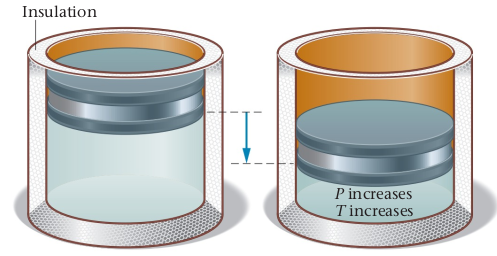
\includegraphics[scale=0.4]{18}
	\end{subfigure}
	\begin{subfigure}[t]{.5\textwidth}
		\centering
		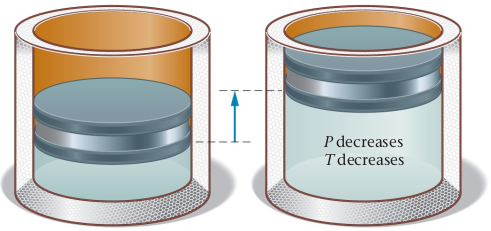
\includegraphics[scale=0.4]{19}
	\end{subfigure}
\end{figure}